In this Chapter we give an overview of functionality contained in the {\tt amrex/Src/AmrCore} source code.
This directory contains source code for the following:
\begin{itemize}
\item Storing information about the grid layout and processor distribution mapping
at each level of refinement.
\item Functions to create grids at different levels of refinement, including tagging
operationrs.
\item Operations on data at different levels of refinement, such as interpolation and
restriction operators.
\item Flux registers used to store and manipulate fluxes at coarse-fine interfaces.
\item Particle support for AMR.
\end{itemize}
There is another source directory, {\tt amrex/Src/Amr/}, which contains
additional classes used to manage the time-stepping for AMR simulations.
However, it is possible to build a fully adaptive, subcycling-in-time simulation code
without these additional classes.

In this Chapter, we restrict our use to the {\tt amrex/Src/AmrCore} source code
and present a tutorial that performs an adaptive, subcycling-in-time simulation
of the advection equation for a passively advected scalar.
The accompanying tutorial code is available in {\tt amrex/Tutorials/Amr/Advection\_AmrCore}
with build/run directory {\tt Exec/SingleVortex}.  In this example, the velocity
field is a specified function of space and time, such that an initial
Gaussian profile is displaced but returns to its original configuration at the final time.
The boundary conditions are periodic and we use a refinement ratio of $r=2$ between each 
AMR level.  The results of the simulation in two-dimensions are depicted in 
Figure \ref{fig:Adv}.
\begin{figure}
  \centering
  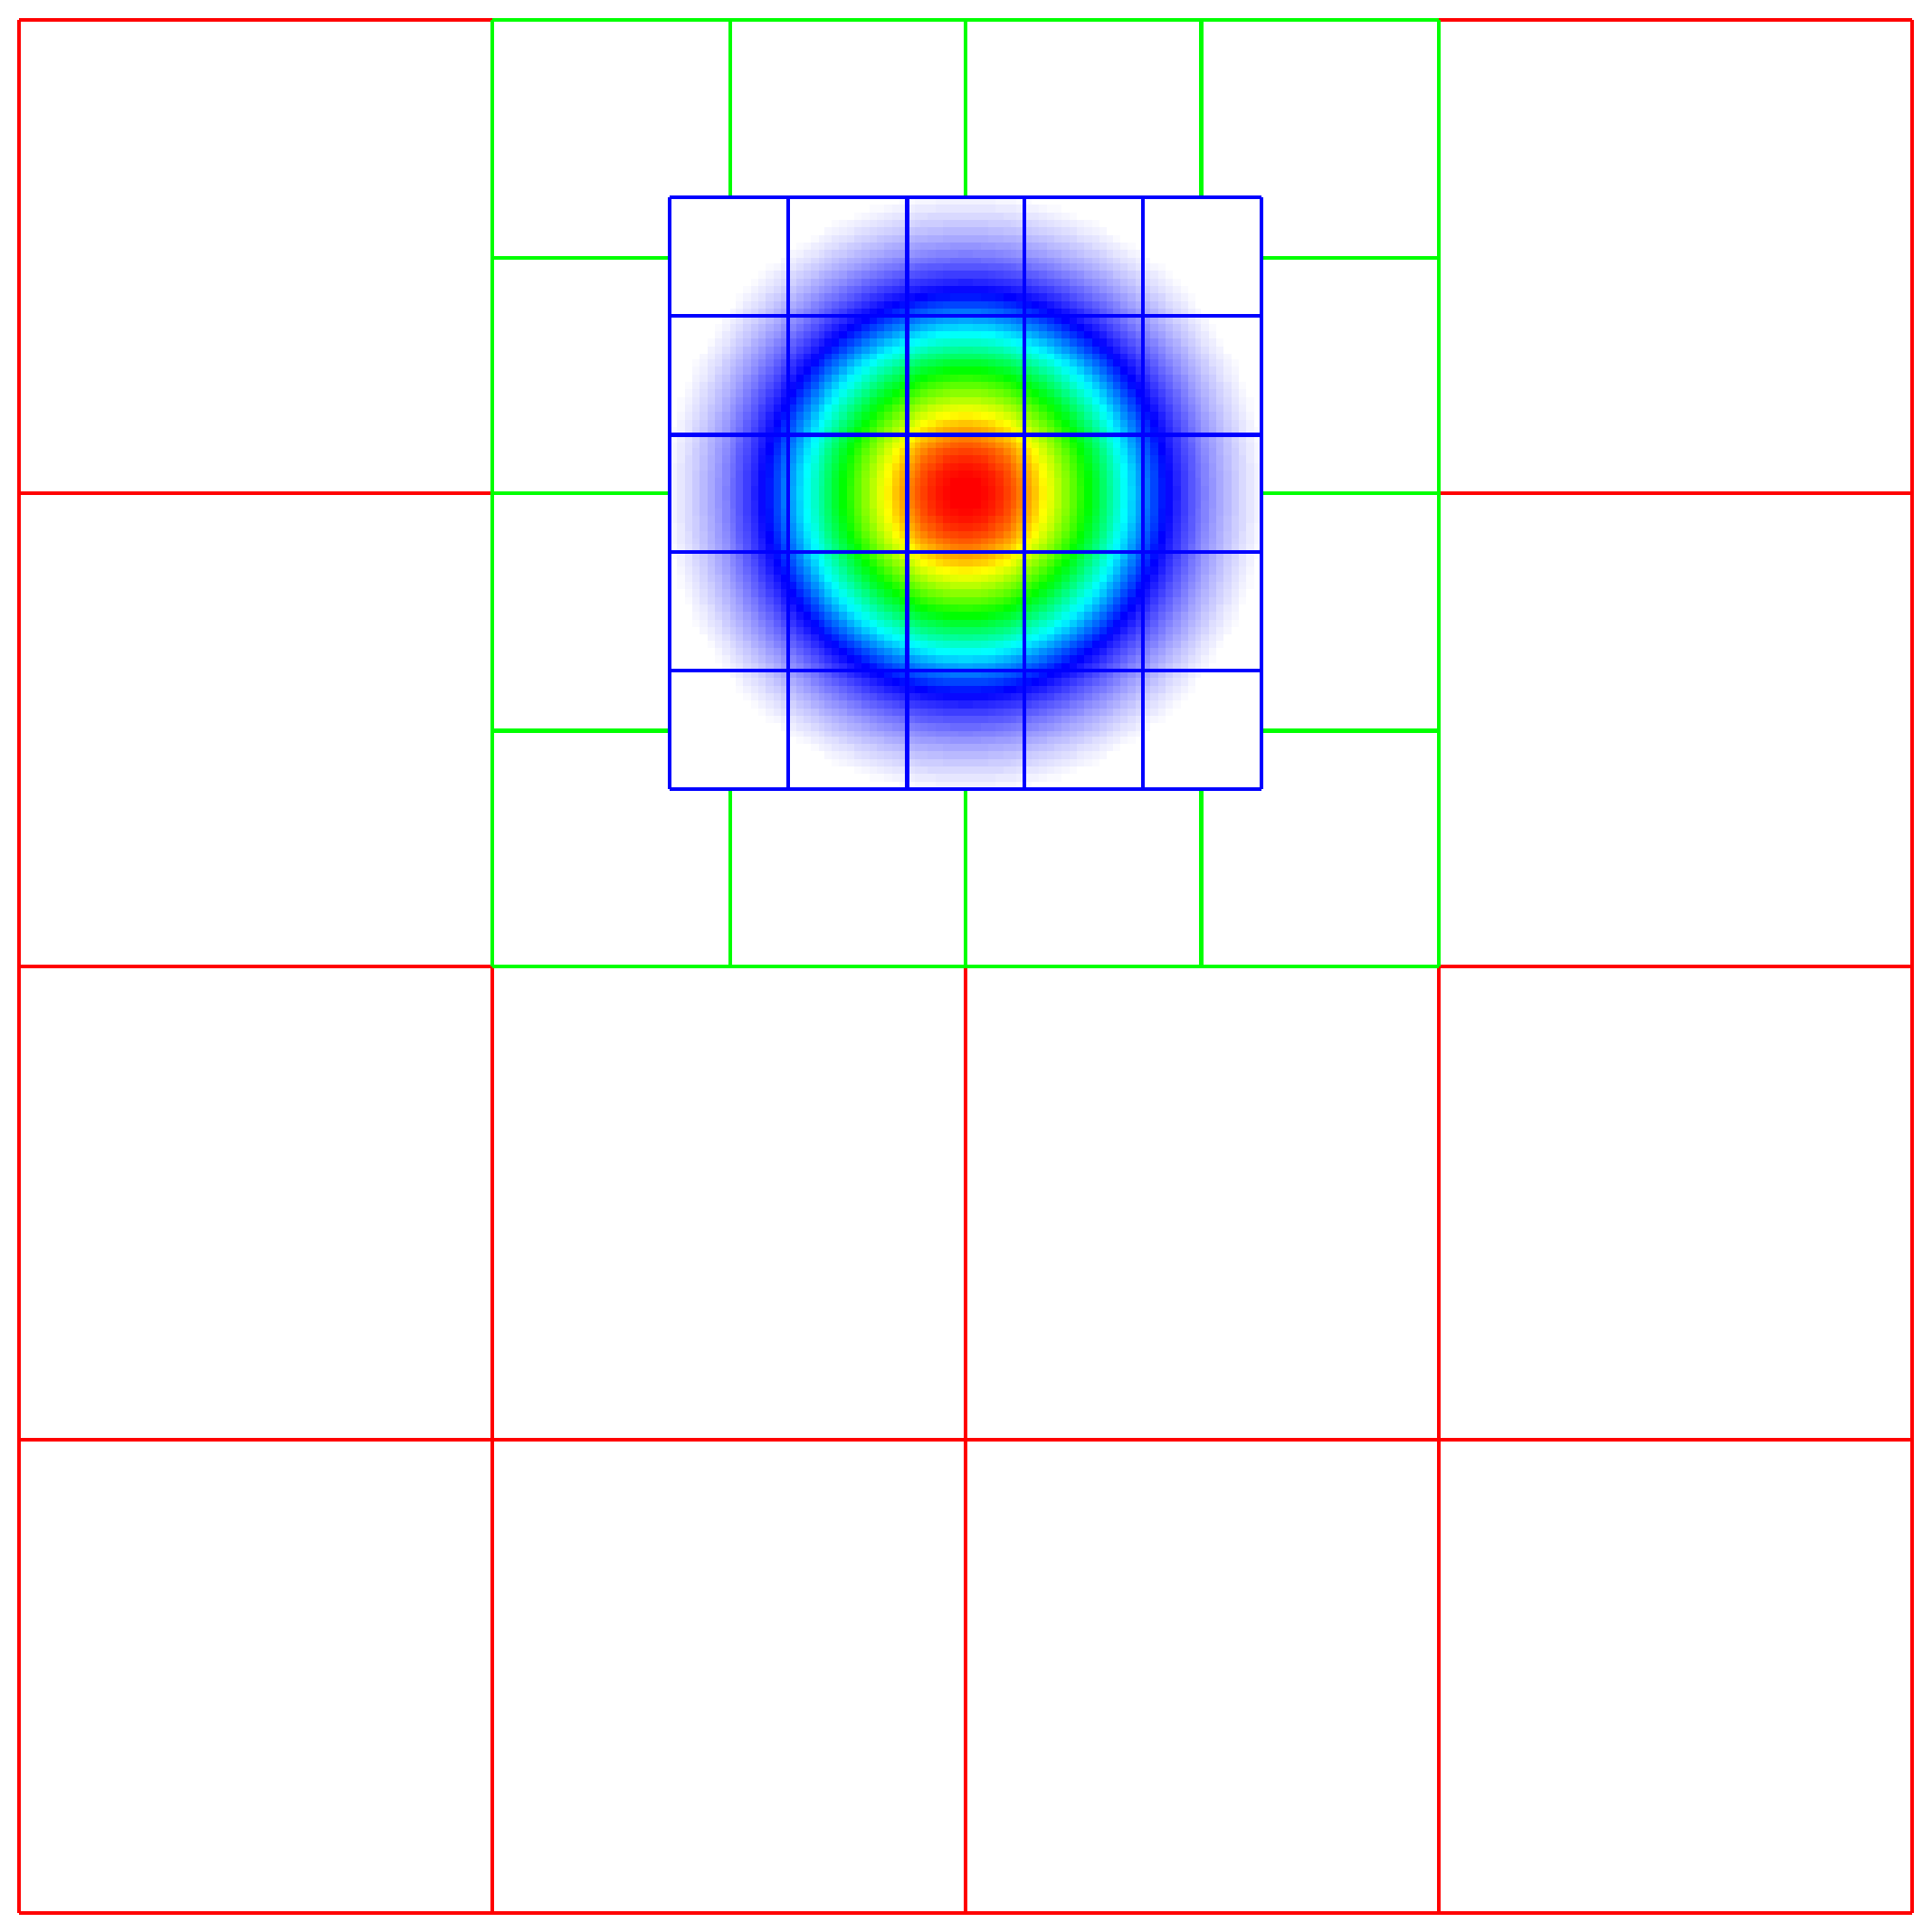
\includegraphics[width=1in]{./AmrCore/figs/Adv1.pdf}
  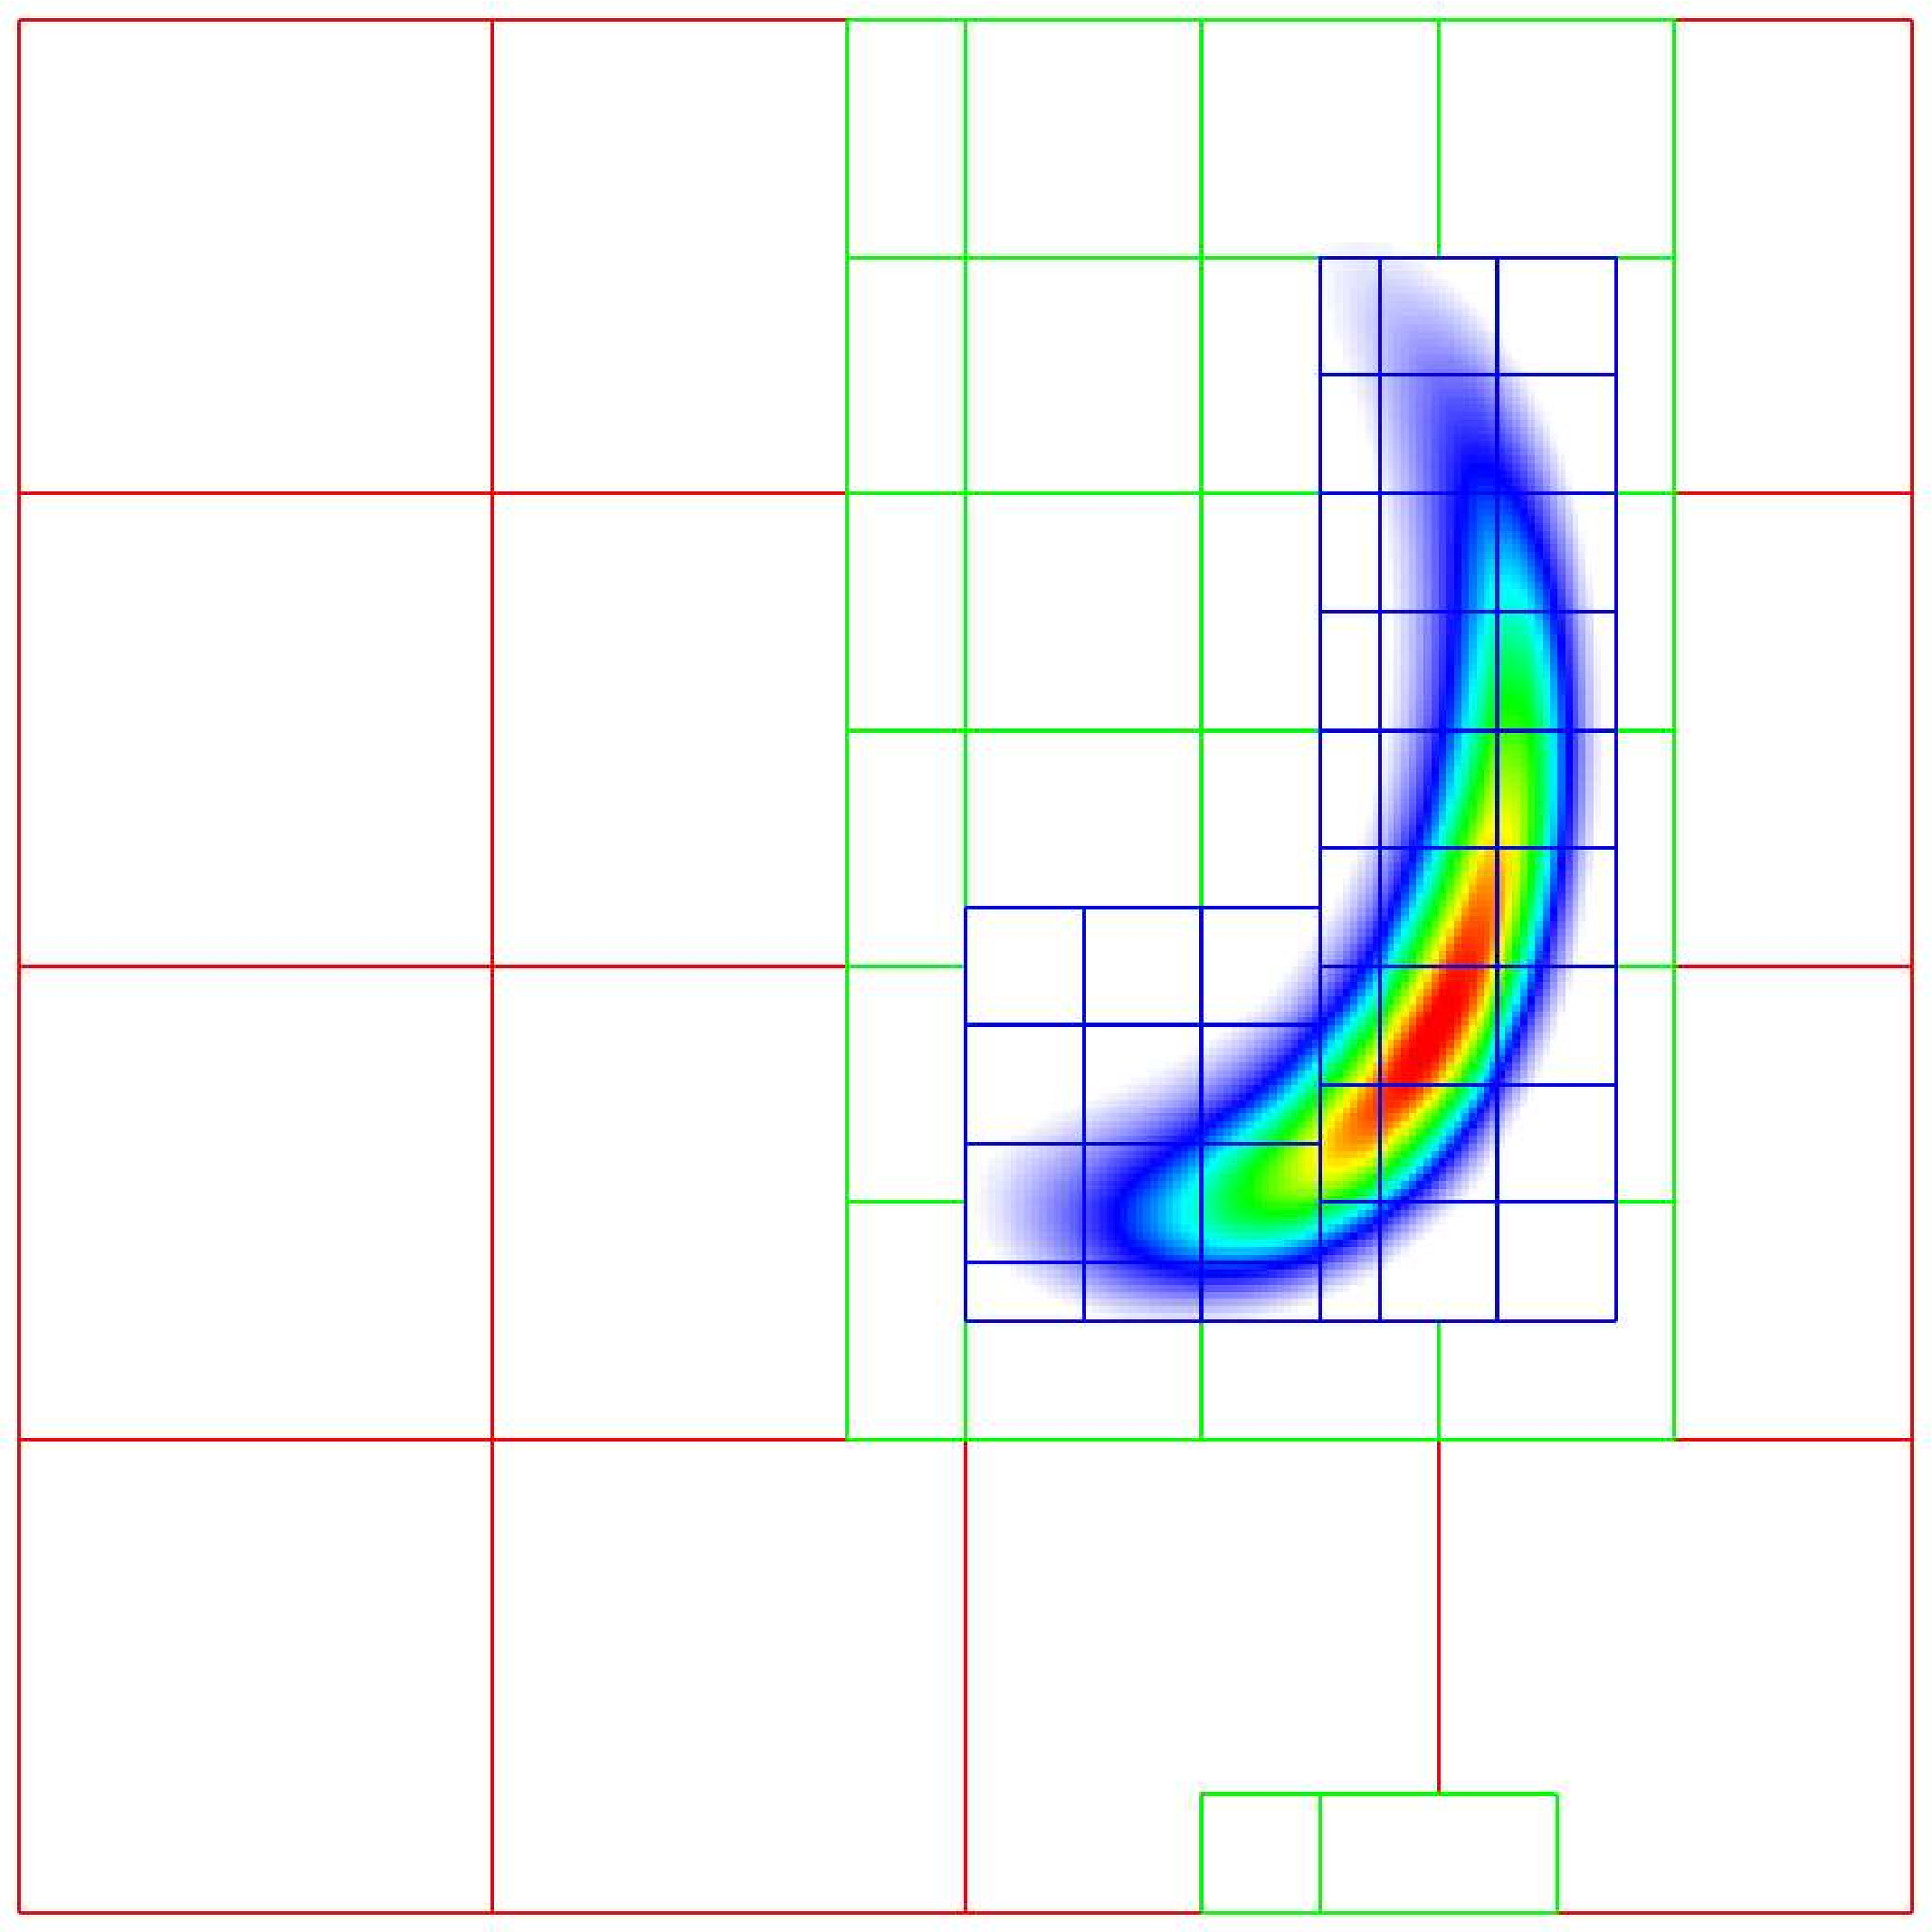
\includegraphics[width=1in]{./AmrCore/figs/Adv2.pdf}
  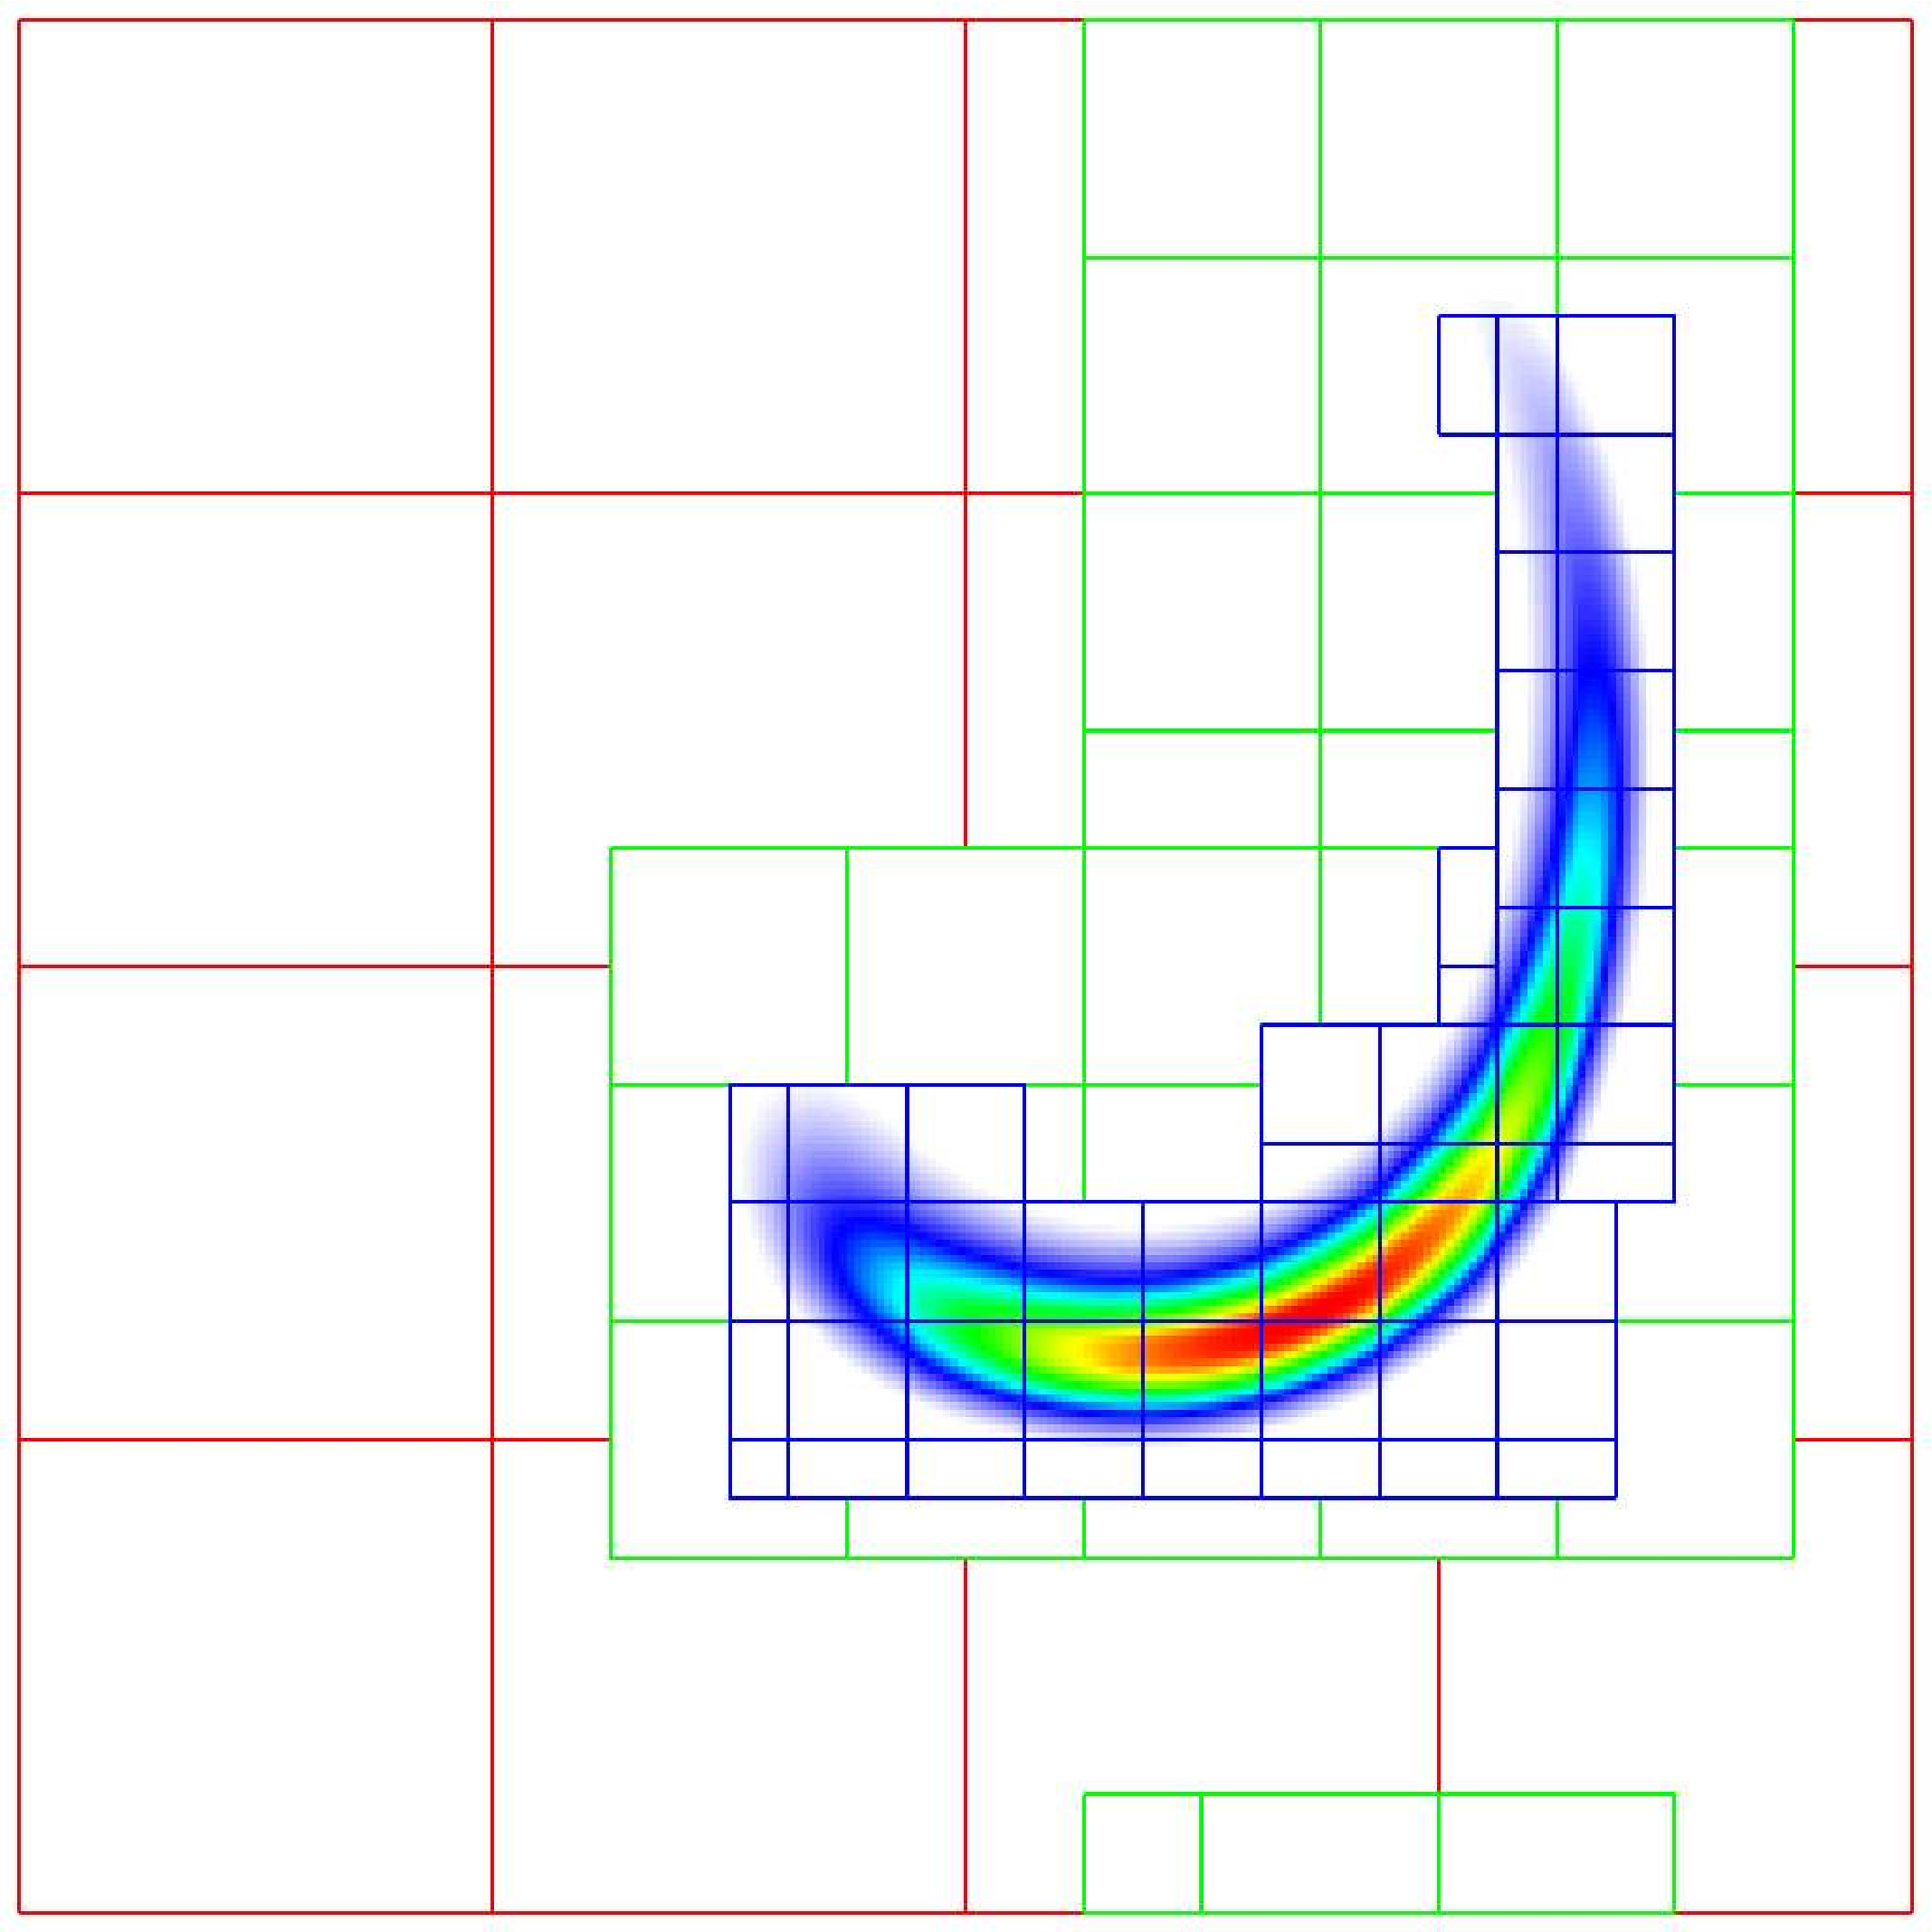
\includegraphics[width=1in]{./AmrCore/figs/Adv3.pdf}
  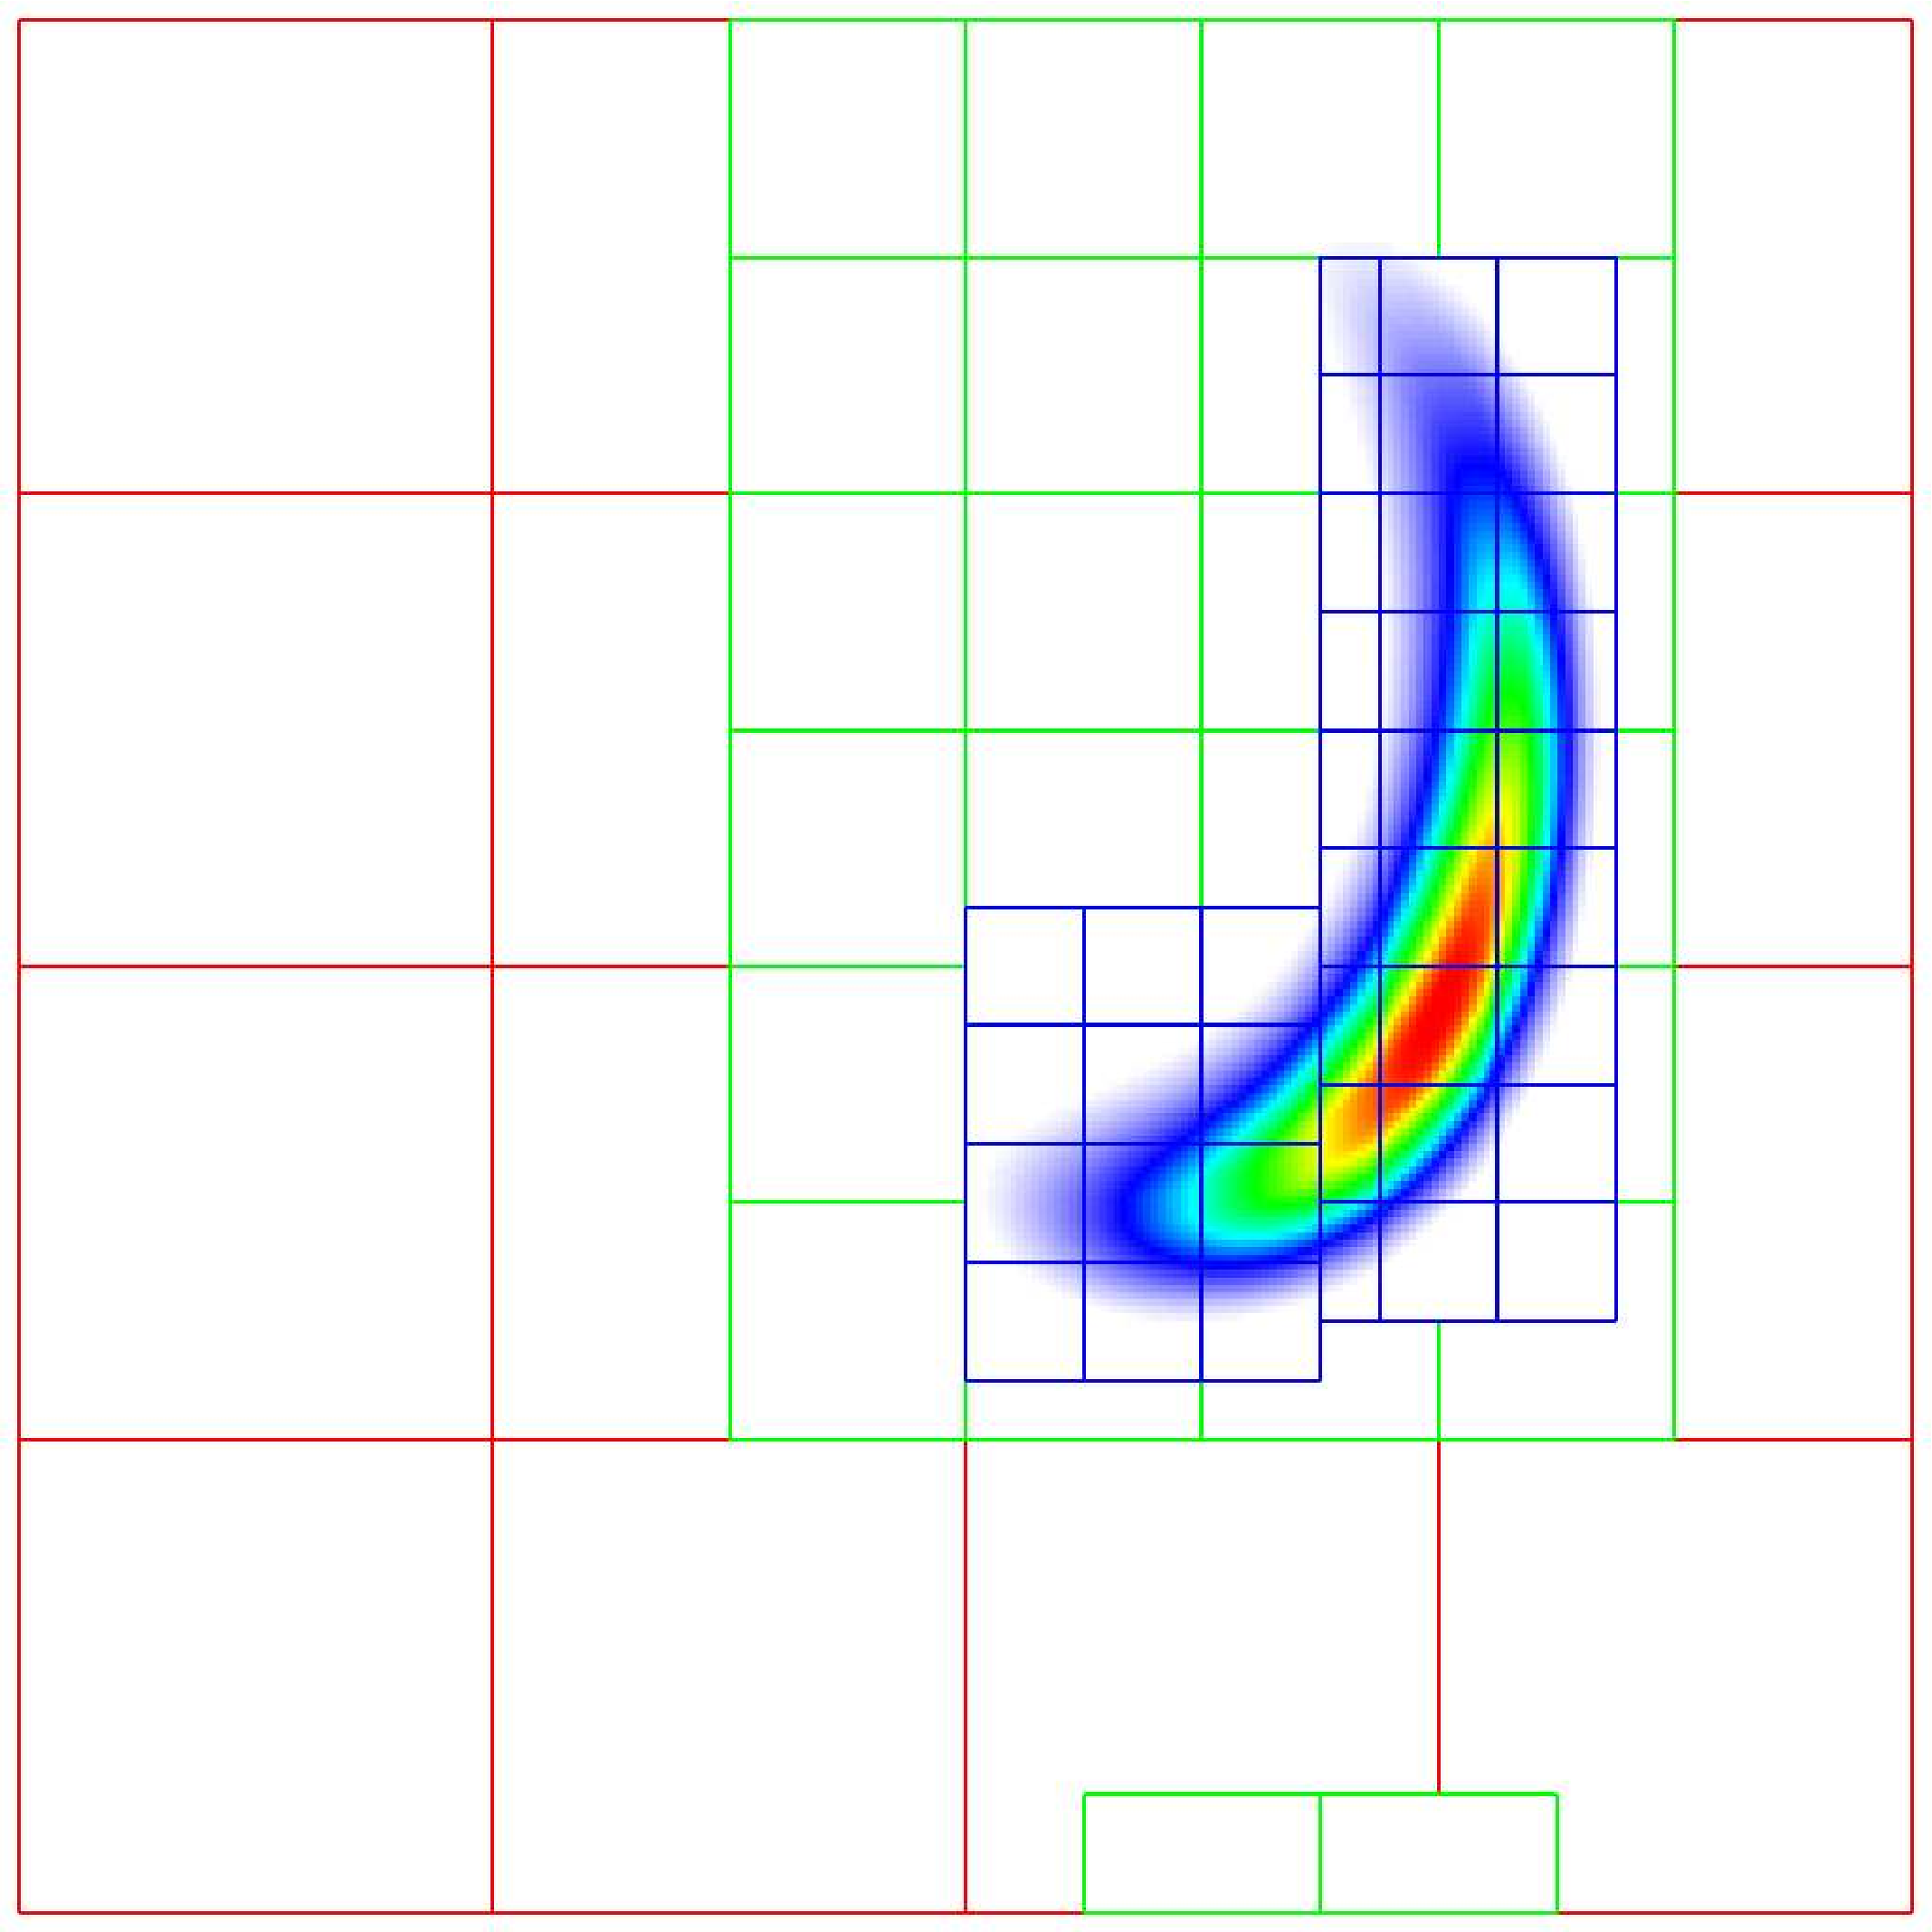
\includegraphics[width=1in]{./AmrCore/figs/Adv4.pdf}
  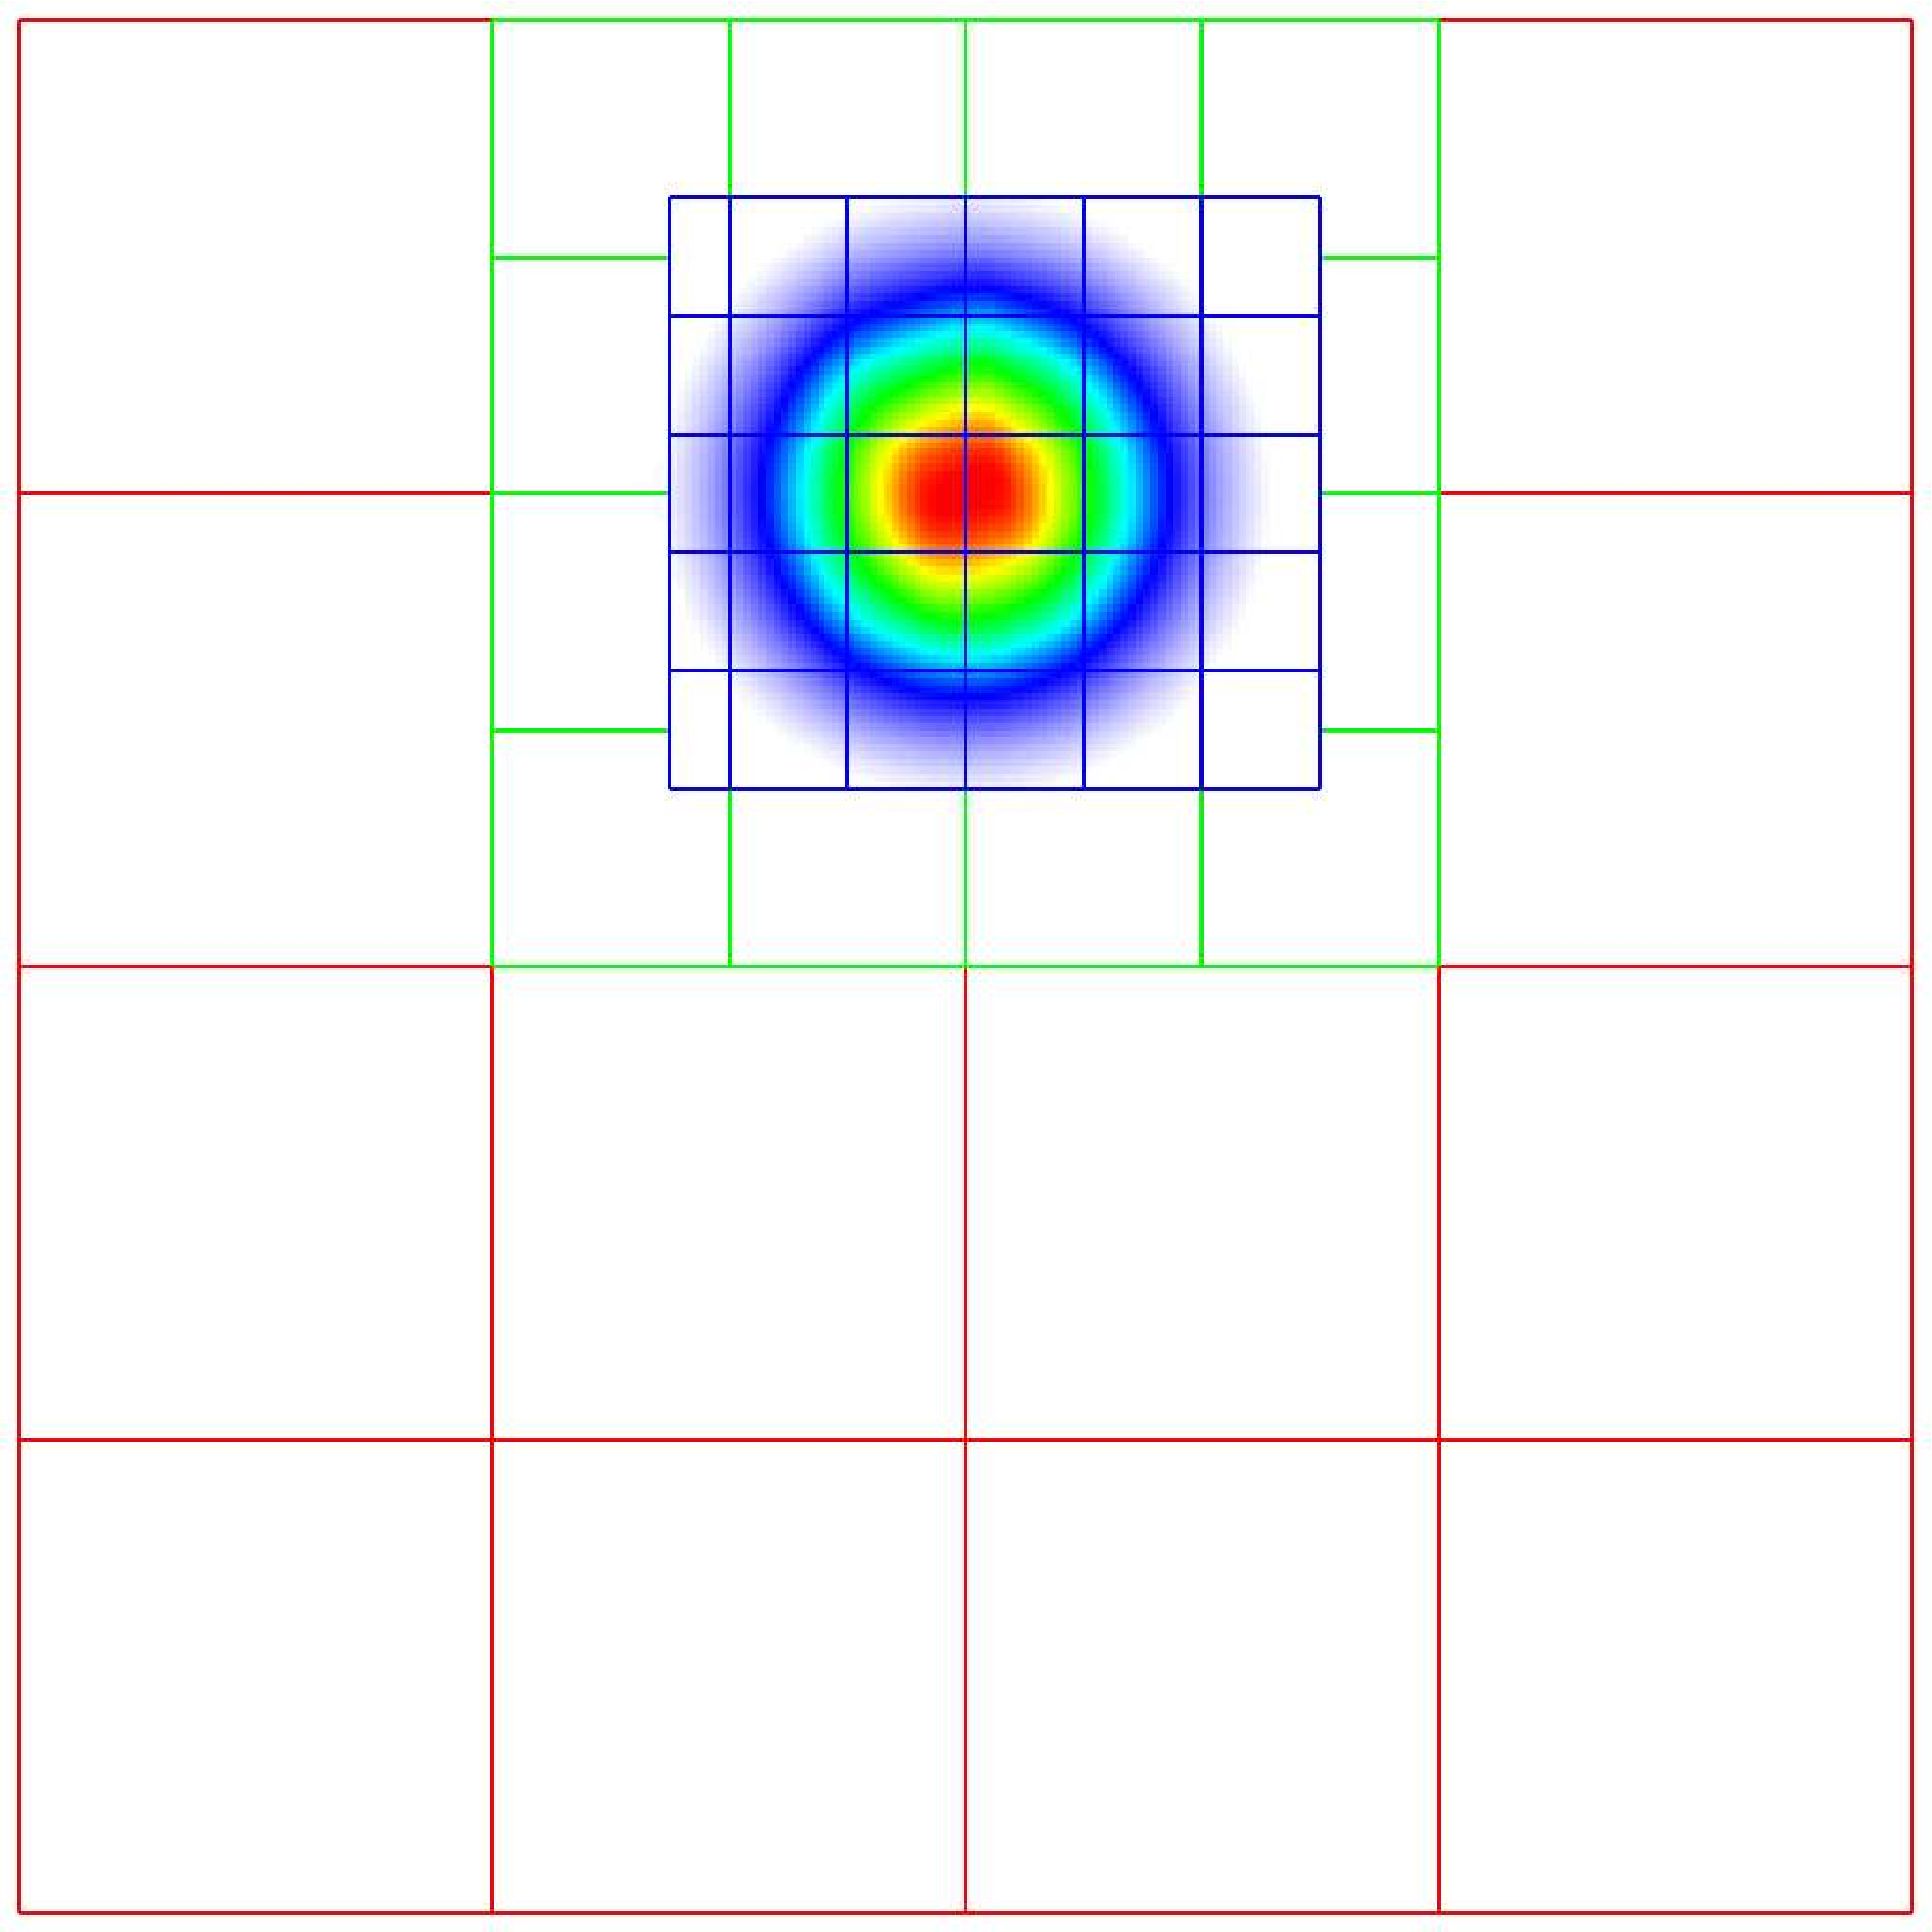
\includegraphics[width=1in]{./AmrCore/figs/Adv5.pdf}
  \caption{\label{fig:Adv} Time sequence ($t=0,0.5,1,1.5,2$~s) of advection of a Gaussian profile using the 
{\tt SingleVortex} tutorial.  The red, green, and blue boxes indicate grids at AMR levels $\ell=0,1$, and $2$.}
\end{figure}

\section{The Advection Equation}
We seek to solve the advection equation on a multi-level, adaptive grid structure:
\begin{equation}
\frac{\partial\phi}{\partial t} = -\nabla\cdot(\phi{\bf U}).
\end{equation}
The velocity field is a specified divergence-free (so the flow field is incompressible)
function of space and time.  The initial scalar field is a
Gaussian profile.  To integrate these equations on a given level, we use a simple conservative update,
\begin{equation}
\frac{\phi_{i,j}^{n+1}-\phi_{i,j}^n}{\Delta t} = \frac{(\phi u)_{i+\myhalf,j}^{n+\myhalf}-(\phi u)_{i-\myhalf,j}^{n+\myhalf}}{\Delta x} + \frac{(\phi v)_{i,j+\myhalf}^{n+\myhalf} - (\phi v)_{i,j-\myhalf}^{n+\myhalf}}{\Delta y},
\end{equation}
where the velocities on faces are prescribed functions of space and time, and the scalars on faces
are computed using a Godunov advection integration scheme.  The fluxes in this case are the face-centered,
time-centered ``$\phi u$'' and ``$\phi v$'' terms.

We use a subcycling-in-time approach where finer levels are advanced with smaller
time steps than coarser levels, and then synchronization is later performed between levels.
More specifically, the multi-level procedure can most
easily be thought of as a recursive algorithm in which, to advance level $\ell$,
$0\le\ell\le\ell_{\rm max}$, the following steps are taken:
\begin{itemize}
\item Advance level $\ell$ in time by one time step, $\Delta t^{\ell}$, as if it is
the only level.  If $\ell>0$, obtain boundary data (i.e. fill the level $\ell$ ghost cells)
using space- and time-interpolated data from the grids at $\ell-1$ where appropriate.
\item If $\ell<\ell_{\rm max}$
\begin{itemize}
\item Advance level $(\ell+1)$ for $r$ time steps with $\Delta t^{\ell+1} = \frac{1}{r}\Delta t^{\ell}$.
\item Synchronize the data between levels $\ell$ and $\ell+1$.
\end{itemize}
\end{itemize}
Specifically, for a 3-level simulation, depicted graphically in Figure \ref{fig:subcycling}:
\begin{enumerate}
\item Integrate $\ell=0$ over $\Delta t$.
\item Integrate $\ell=1$ over $\Delta t/2$.
\item Integrate $\ell=2$ over $\Delta t/4$.
\item Integrate $\ell=2$ over $\Delta t/4$.
\item Synchronize levels $\ell=1,2$.
\item Integrate $\ell=1$ over $\Delta t/2$.
\item Integrate $\ell=2$ over $\Delta t/4$.
\item Integrate $\ell=2$ over $\Delta t/4$.
\item Synchronize levels $\ell=1,2$.
\item Synchronize levels $\ell=0,1$.
\end{enumerate}
%%%%%%%%%%%%%%%%%%%%%%%%%%%%%
\begin{figure}[htb]
\begin{center}
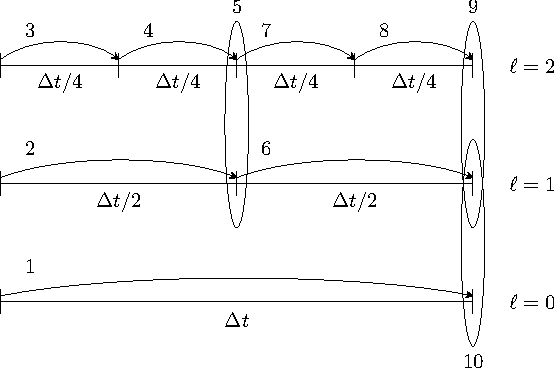
\includegraphics[width=4in]{./AmrCore/figs/subcycling.pdf}
\caption{\label{fig:subcycling} Schematic of subcycling-in-time algorithm.}
\end{center}
\end{figure}
%%%%%%%%%%%%%%%%%%%%%%%%%%%%%
For the scalar field, we keep track volume and time-weighted fluxes at coarse-fine interfaces.
We accumulate area and time-weighted fluxes in {\tt FluxRegister} objects, which can be
thought of as special boundary {\tt FABset}s associated with coarse-fine interfaces.

The idea behind the level $\ell/(\ell+1)$ synchronization step is to correct for sources of mismatch in the composite solution:
\begin{enumerate}
\item The data at level $\ell$ that underlie the level  $\ell+1$ data are not synchronized with the level $\ell+1$ data.
This is simply corrected by overwriting covered coarse cells to be the average of the overlying fine cells.
\item The area and time-weighted fluxes from the level $\ell$ faces and the level $\ell+1$ faces
do not agree at the $\ell/(\ell+1)$ interface, resulting in a loss of conservation.  
The remedy is to modify the solution in the coarse cells immediately next to the coarse-fine interface
to account for the mismatch stored in the flux register (computed by taking the coarse-level divergence of the
flux register data).
\end{enumerate}

\section{{\tt AmrMesh} and {\tt AmrCore}}

For single-level simulations
(see e.g., {\tt amrex/Tutorials/Basic/HeatEquation\_EX1\_C/main.cpp})
the user needs to build {\tt Geometry}, {\tt DistributionMapping},
and {\tt BoxArray} objects associated with the simulation.  For simulations
with multiple levels of refinement, the {\tt AmrMesh} class can be thought
of as a container to store arrays of these objects (one for each level), and
information about the current grid structure.

{\tt amrex/Src/AmrCore/AMReX\_AmrMesh.cpp/H} contains the {\tt AmrMesh} class.
The protected data members are:
\begin{lstlisting}[language=cpp]
protected:
    int            verbose;
    int            max_level;       // Maximum allowed level.
    Array<IntVect> ref_ratio;       // Refinement ratios [0:finest_level-1]

    int            finest_level;    // Current finest level.

    Array<int>     n_error_buf;     // Buffer cells around each tagged cell.
    Array<int>     blocking_factor; // Blocking factor in grid generation 
                                    // (by level).
    Array<int>     max_grid_size;   // Maximum allowable grid size (by level).
    Real           grid_eff;        // Grid efficiency.
    int            n_proper;        // # cells required for proper nesting.

    bool use_fixed_coarse_grids;
    int  use_fixed_upto_level;
    bool refine_grid_layout;        // chop up grids to have the number of 
                                    // grids no less the number of procs

    Array<Geometry>            geom;
    Array<DistributionMapping> dmap;
    Array<BoxArray>            grids;    
\end{lstlisting}

{\tt AMReX\_AmrCore.cpp/H} contains the class {\tt AmrCore}, which is derived from
the {\tt AmrMesh} class.

\section{{\tt Cluster}, {\tt ErrorList}, and {\tt TagBox}}

\section{{\tt Interpolater}}

{\tt AMReX\_Interpolater.cpp/H} contains the virtual base class {\tt Interpolater}, which provides
an interface for coarse-to-fine spatial interpolation operators.  Within {\tt AMReX\_Interpolater.cpp/H}
are the derived classes:
\begin{itemize}
\item {\tt NodeBilinear}
\item {\tt CellBilinear}
\item {\tt CellConservativeLinear}
\item {\tt CellConservativeProtected}
\item {\tt CellQuadratic}
\item {\tt PCInterp}
\item {\tt CellConservativeQuartic}
\end{itemize}
The fortran routines that perform the actual work associated with {\tt Interpolater} are 
contained in the files {\tt AMReX\_INTERP\_F.H} and {\tt AMReX\_INTERP\_xD.F}.

\section{{\tt FillPatchUtil}}
\label{sec:amrcore:fillpatch}

{\tt AMReX\_FillPatchUtil.cpp/H} contains as assortment of functions to check for proper nesting
and to help with interpolation.

\section{{\tt FluxRegister}}

{\tt AMReX\_FluxRegister.cpp/H} contains the class {\tt FluxRegister}, which is derived from
the class {\tt BndryRegister} (in {\tt Src/Boundary/AMReX\_BndryRegister}).
In the most general terms, a {\tt FluxRegister} is a special type of {\tt BndryRegister} that
stores and manipulates fluxes at coarse-fine interfaces.
A simple usage scenario comes from a conservative discretization of a hyperbolic system:
\begin{equation}
\frac{\partial\phi}{\partial t} = \nabla\cdot{\bf F}
\rightarrow
\frac{\phi_{i,j}^{n+1}-\phi_{i,j}^n}{\Delta t} = \frac{F_{i+\myhalf,j}-F_{i-\myhalf,j}}{\Delta x} + \frac{F_{i,j+\myhalf} - F_{i,j-\myhalf}}{\Delta y}.
\end{equation}
Consider a two-level, two-dimensional simulation.  A standard methdology for advancing the solution in 
time is to first advance the coarse grid solution ignoring the fine level, and then advance the fine 
grid solution using the coarse level only to supply boundary conditions.  At the coarse-fine interface, 
the area weighted fluxes from the fine grid advance do not in general match the underlying flux from 
the coarse grid face, resulting in a lack of conservation.  Note that for subcycling-in-time algorithms
(where for each coarse grid advance, the fine grid is advanced $r$ times using a coarse grid time step 
reduced by a factor of $r$, where $r$ is the refinement ratio), the coarse grid flux must 
be compared to the area {\it and} time-weighted fine grid fluxes.  A {\tt FluxRegister} accumulates 
and ultimately stores the net difference in fluxes between the coarse grid and fine grid advance over 
each face over a given coarse time step.  The simplest possible synchronization step is to modify
the coarse grid solution in coarse cells immediately adjacent to the coarse-fine interface are updated
to account for the mismatch stored in the {\tt FluxRegister}.

The fortran routines that perform the actual work associated with {\tt FluxRegister} are 
contained in the files {\tt AMReX\_FLUXREG\_F.H} and {\tt AMReX\_FLUXREG\_xD.F}.

\section{{\tt AmrParticles} and {\tt AmrParGDB}}

The {\tt AmrCore/} directory contains derived class for dealing with particles 
in a multi-level framework.  The description of the base classes
are given in Chapter \ref{Chap:Particles}.

{\tt AMReX\_AmrParticles.cpp/H} contains the classes {\tt AmrParticleContainer}
and {\tt AmrTracerParticleContainer}, which are derived from the classes
{\tt ParticleContainer} (in {\tt Src/Particle/AMReX\_Particles})
and {\tt TracerParticleContainer} (in {\tt Src/Particle/AMReX\_TracerParticles}).

{\tt AMReX\_AmrParGDB.cpp/H} contains the class {\tt AmrParGDB}, which is derived from
the class {\tt ParGDBBase} (in {\tt Src/Particle/AMReX\_ParGDB}).

\section{{\tt Advection\_AmrCore} Example}
This example uses the class {\tt AmrAdv}, which is derived from the class {\tt AmrCore} 
(which is derived from {\tt AmrMesh}).  The function definitions are given in {\tt AmrAdv.H}.
The function implementations are split among 5 files 
({\tt AmrAdv.cpp}, {\tt AmrAdvInit.cpp}, {\tt AmrAdvEvolve.cpp}, {\tt AmrAdvIO.cpp}, and {\tt AmrAdvError.cpp}).

Here is a high-level pseudo-code of the flow of the program:
\begin{lstlisting}[language=cpp]
/* Advection_AmrCore Pseudocode */
main()
  AmrAdv amradv; // build an AmrAdv object
  amradv.InitData()  // initialize data all all levels
    AmrCore::InitFromScratch()
      AmrMesh::MakeNewGrids()
	AmrMesh::MakeBaseGrids() // define level 0 grids
	AmrAdv::MakeNewLevelFromScratch()
          /* allocate phi_old, phi_new, t_new, and flux registers */
          initdata()  // fill phi
	if (max_level > 0) {
          do {
  	    AmrMesh::MakeNewGrids()
	      /* construct next finer grid based on tagging criteria */
 	    AmrAdv::MakeNewLevelFromScratch()
              /* allocate phi_old, phi_new, t_new, and flux registers */
              initdata()  // fill phi
	  } (while (finest_level < max_level);
        }
  amradv.Evolve()
    loop over time steps {
      ComputeDt()
      timeStep() // advance a level
        /* check regrid conditions and regrid if necessary */
        Advance()
          /* copy phi into a multifab and fill ghost cells */
          /* advance phi */
          /* update flux registers */
        if (lev < finest_level) {
          timeStep() // recursive call to advance the next-finer level "r" times
            /* check regrid conditions and regrid if necessary */
            Advance()
              /* copy phi into a multifab and fill ghost cells */
              /* advance phi */
              /* update flux registers */
          reflux() // synchronize lev and lev+1 using fluxregister divergence
          AverageDown() // set covered coarse cells to be the average of fine
        }
    }
\end{lstlisting}
